\documentclass{article}
\usepackage[a4paper, tmargin=1in, bmargin=1in]{geometry}
\usepackage[utf8]{inputenc}
\usepackage{graphicx}
\usepackage{parskip}
\usepackage{pdflscape}
\usepackage{listings}
\usepackage{pdflscape}

\title{Microprocessors Project 2 - IITB-RISC Pipeline}
\author{Meet Udeshi - 14D070007\\
Arka Sadhu - 140070011\\
Shruti Hiray - 14D070016\\
Ravi Sharma - 14D070055
}
\date{November 2016}

\begin{document}
\maketitle                      
\pagebreak
\begin{landscape}
    \section*{Datapath}
    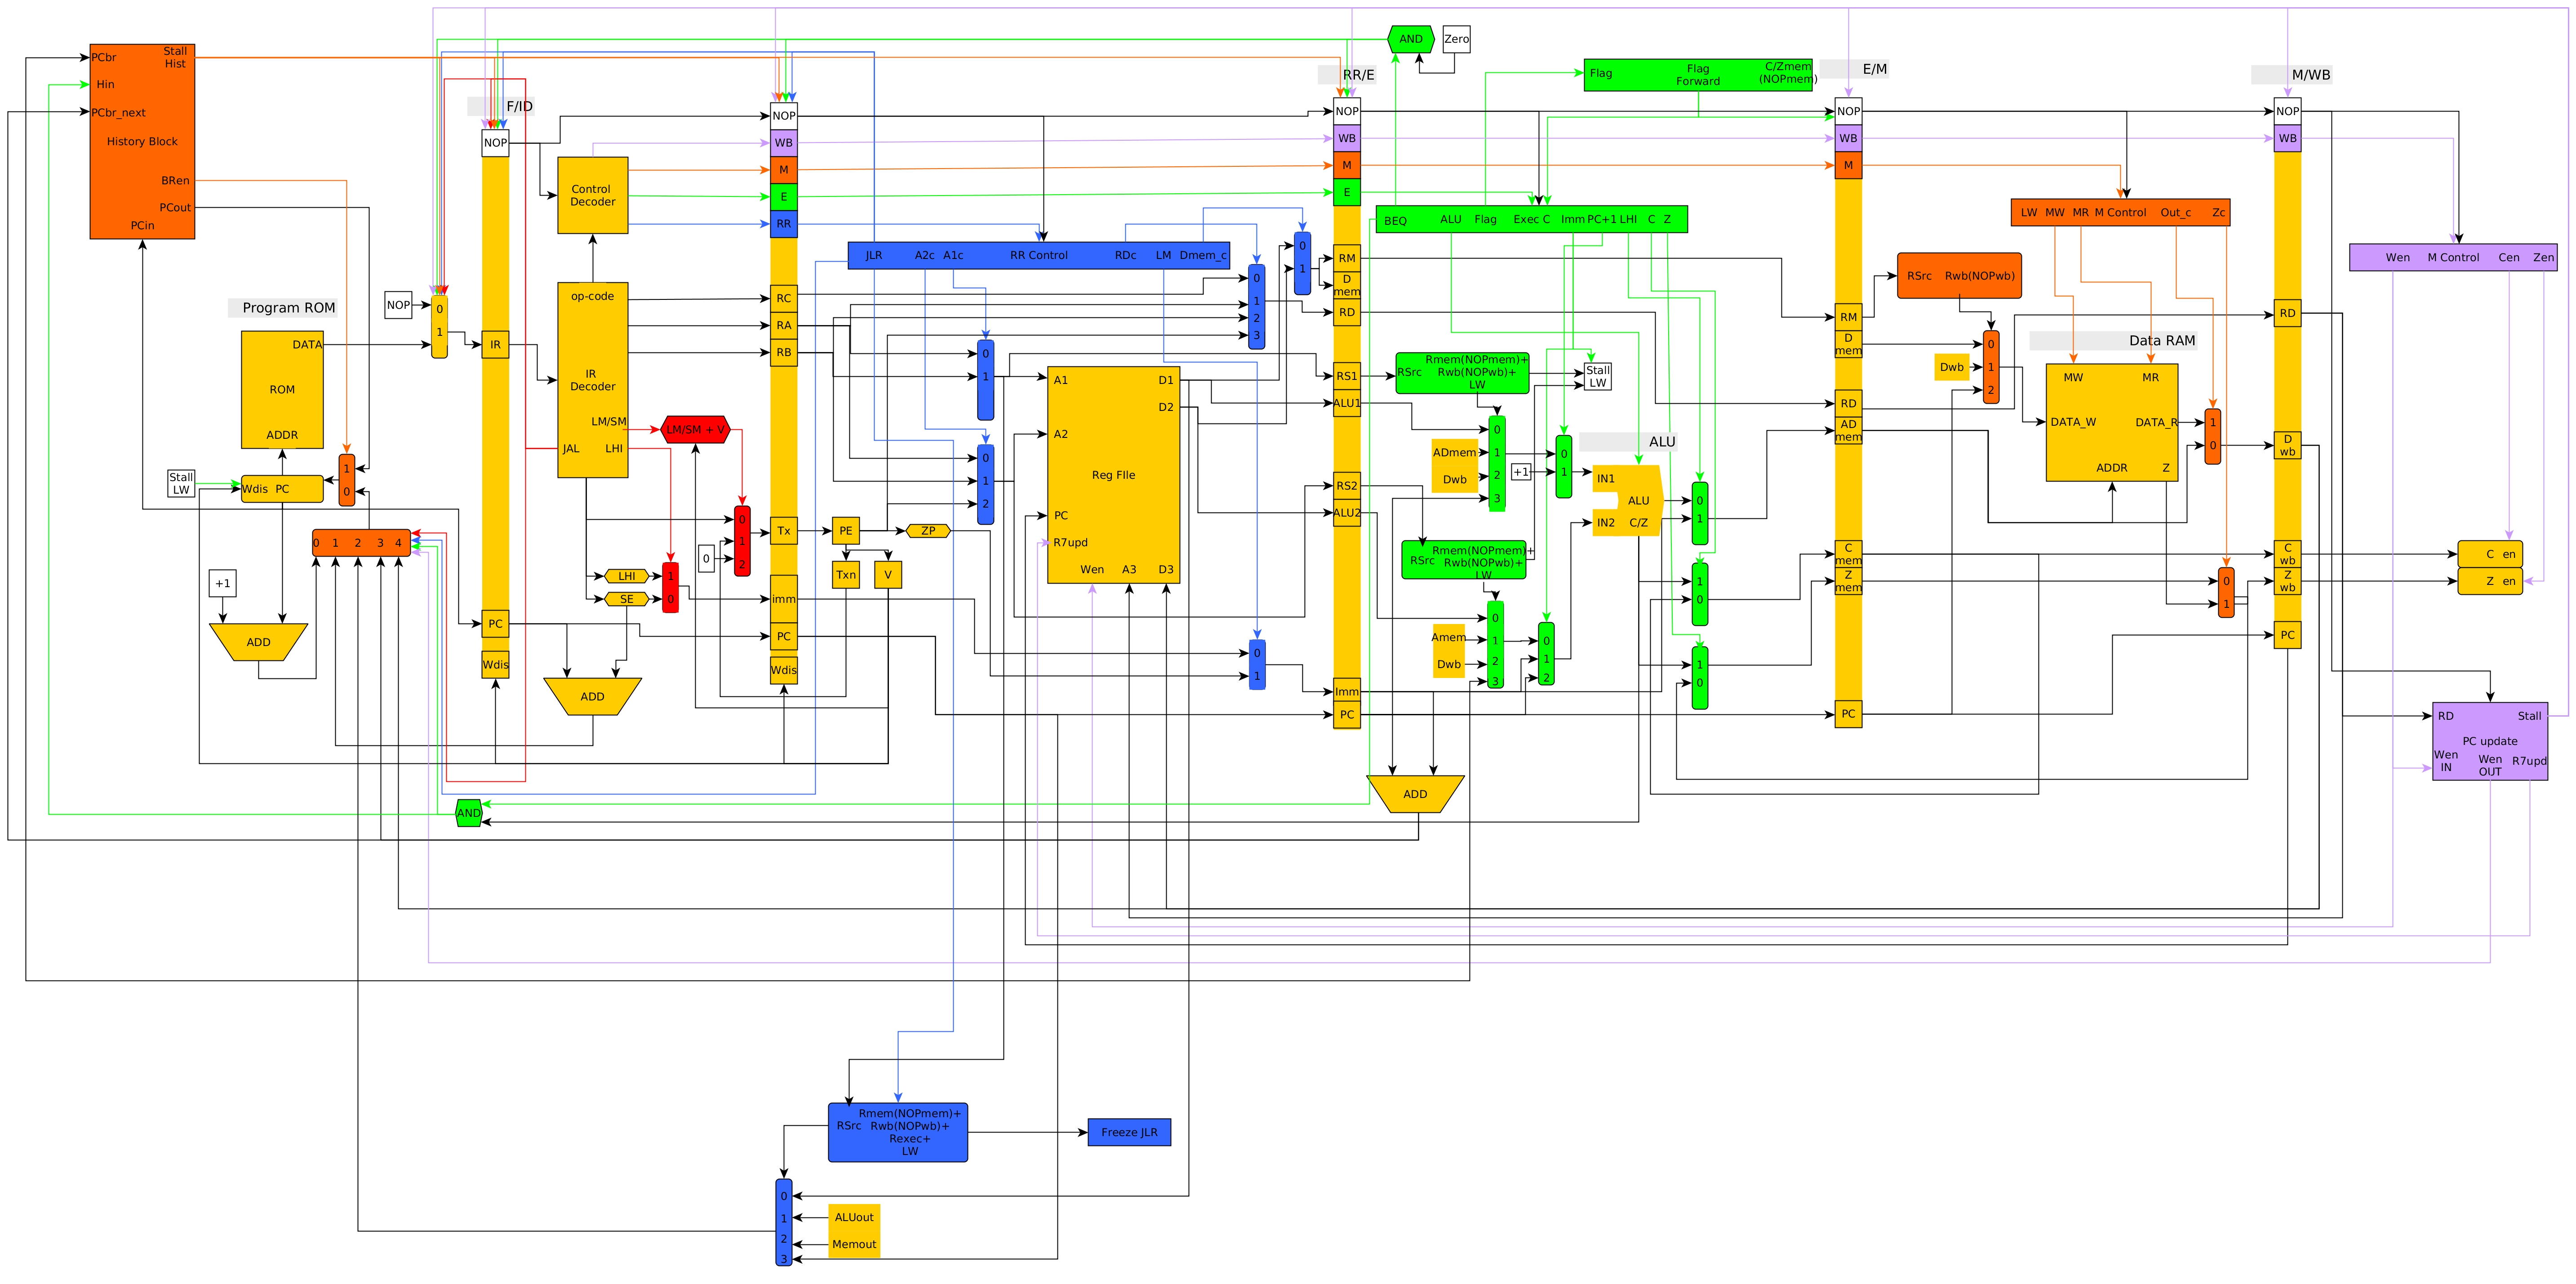
\includegraphics[scale=0.11]{pipeline}
\end{landscape}
\section*{List of Control Signals}

\subsection*{NOP bit}

NOP bit will be active low, so for each instruction, NOP is high. When NOP is
low then that instruction will not be executed.

NOP bit controls the output of individual control decoders of each stage.
If NOP bit is set, all control signals are disabled for that stage.

\subsection*{RR Control}

\begin{tabular}{|l|l|}
\hline
\textbf{Control Signal} & \textbf{Description}\\
\hline
\textbf{JLR} & Controls stall for JLR instruction. \\
             & Goes to PC load mux and sets NOP of previous stages.\\
\hline
\textbf{A1c/A2c} & Controls mux for A1/A2 input of Register File.\\
\hline
\textbf{RDc} & Controls mux for RD(destination register) address.\\
\hline
\textbf{LM/SM} & Controls ALUI2 mux for passing Zero-Padded-PE output to ALU.\\
\hline
\textbf{Dmem} & Controls mux for choosing Dmem and RM for store operations.\\
\hline
\end{tabular}

\subsection*{Exec Control}

\begin{tabular}{|l|l|}
\hline
\textbf{Control Signal} & \textbf{Description}\\
\hline
\textbf{BEQ} & Controls stall for BEQ instruction if ALU gives zero.\\
             & Goes to PC load mux and sets NOP of previous stages.\\
\hline
\textbf{ALU\_c} & Controls operation to be done by ALU (ADD/NAND/XOR).\\
\hline
\textbf{Flag} & Enables flag forwarding block.\\
\hline
\textbf{Imm} & Controls mux for ALUI2 to choose Immediate data.\\
\hline
\textbf{PC1} & Controls mux for ALUI1 to choose constant "+1".\\
             & Controls mux for ALUI2 to choose PC.\\
\hline
\textbf{LHI} & Controls mux for ADmem to send ALUO or Immediate data(for LHI).\\
\hline
\textbf{C/Z} & Controls flag muxes to pass flags from ALU if instruction sets them.\\

\hline
\end{tabular}


\subsection*{Mem Control}

\begin{tabular}{|l|l|}
\hline
\textbf{Control Signal} & \textbf{Description}\\
\hline
\textbf{LW} & Goes to Register Forwarding blocks in Exec stage to determine LW stall.\\
\hline
\textbf{MW/MR} & Controls Read/Write enable of RAM.\\
\hline
\textbf{Out\_c} & Controls mux to select RAM data output or ALU output.\\
\hline
\textbf{Zc} & Controls whether Z flag is updated by data read.\\
\hline
\end{tabular}

\subsection*{WB Control}

\begin{tabular}{|l|l|}
\hline
\textbf{Control Signal} & \textbf{Description}\\
\hline
\textbf{Wen} & Enable data write for Register File\\
\hline
\textbf{Cen/Zen} & Enable write for C/Z registers.\\
\hline
\end{tabular}

\pagebreak
\section*{Combinational Blocks}
\subsection*{Forwarding Block}

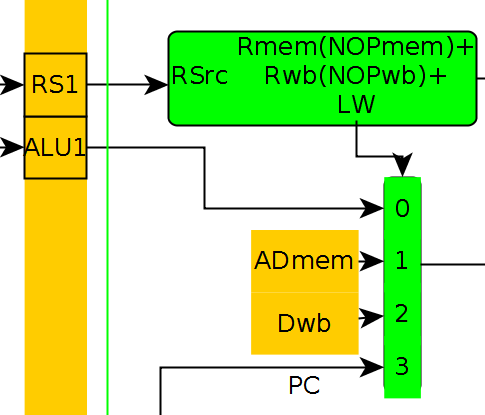
\includegraphics[scale=0.7]{forwarding_block}

This block will compare \textbf{Rsrc} with \textbf{Rmem} and \textbf{Rwb} and
output a control signal for mux to select the corresponding data.
If \textbf{Rsrc} is equal to \textbf{R7}, we need to select the current PC.

Also, if \textbf{LW} is set for Mem stage and \textbf{Rsrc} matches, we need to
stall.

Logic:
    \begin{lstlisting}
        if(Rsrc == R7){
            Out = PC;
        } else {
            if(NOPmem == 0 && Rsrc == Rmem && Wen_mem == 1){
                if (LW == 1) {
                    Stall;
                } else {
                    Out = ADmem;
                }
            } else if(NOPwb == 0 && Rsrc == Rwb && Wen_wb == 1){
                Out = Dwb;
            }
        }

    \end{lstlisting}

\subsection*{LW Stall Block}
It takes input from the 3 forwarding blocks and if we want to stall, it disables
write of all previous pipeline registers(and PC) so they stay in same state, and sets 
\textbf{NOP} bit of \textbf{E/M} pipeline register to send \textbf{NOP} instruction (i.e. stall) to Mem stage.

Current instruction in Exec stage will be recomputed using the forwarding values
obtained from WB stage(which now has \textbf{LW} instruction).
\subsection*{Forwarding Block for jlr and Freeze Logic}

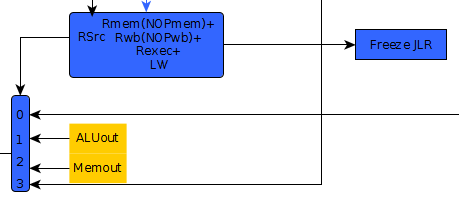
\includegraphics[scale=1]{jlr_freeze_logic}
This works the same as the normal forwarding block except that this is now in the register read stage. It compares
\textbf{Rsrc} with \textbf{Rexec}, \textbf{Rmem} and \textbf{Rwb} and output a control signal for the mux to select
the corresponding data. Similarly if \textbf{Rsrc} is \textbf{R7} we need to select current PC. Also we will have
to output to pipeline freeze logic. We may need to freeze the pipeline sometimes, because we might not have the
required value of the register until the end of the execute stage. This is done by \textbf{freeze\_jlr} which will
disable the write signals for all the Pipeline registers before RegRead, ie DRR and FD will be frozen.
\\ Logic for Data Forwarding if there is JLR.
\begin{lstlisting}

    Out = D1;
    if (Rsrc == R7)
    {
      Out = PC;
    }
    else
    {
      if (NOPexec == 0 && Rsrc == Rexec && Wen_exec==1)
      {
        if(LWexec == 1)
        {
          freeze_jlr;
        }
        else
        {
          out = ALUout;
        }
      }
      elsif (NOPmem == 0 && Rsrc == Rmem && Wen_mem == 1)
      {
        if (LWmem == 1)
        {
          out = Memout;
        }
      }
    }
    \end{lstlisting}

\subsection*{Forwarding Block Inside the Regfile}
We note that there might be cases in which the value of the register in the regfile is updated
by the writeback pipeline register, and at the same time the register is being read by A1 and A2.The
value in the register will be updated at the end of the cycle. Therefore in case A1(or A2) is the
same as A3, we need to do dataforwarding.
Extra logic inside the Register File:
    \begin{lstlisting}
      if (A1 == A3)
      {
        D1 = D3;
      }
      if (A2 == A3)
      {
        D2 = D3;
      }
    \end{lstlisting}


\subsection*{Flag Forwarding Block}

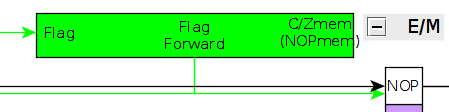
\includegraphics{flag_forward}
Used by \textbf{ADC/ADZ/NDC/NDZ} instructions to determine whether to execute
or change to \textbf{NOP}.

Logic:
    \begin{lstlisting}
        if(NOPmem == 1){
            if(Flag == C && Cmem == 0){
                Dont execute;
            } else if(Flag == Z){
              if (LW == 1)
              {
                Stall;
              }
              else
              {
                if (Zmem = 0)
                {
                  Dont execute;
                } 
              }
            }
        }
    \end{lstlisting}

If we decide to not execute, the Exec state's control decoder is disabled, and
\textbf{NOP} bit is set in \textbf{E/M} pipeline register to send \textbf{NOP}
instruction. This means the instruction will not execute further.

\pagebreak
\subsection*{LM/SM Initialisation and Freeze logic}

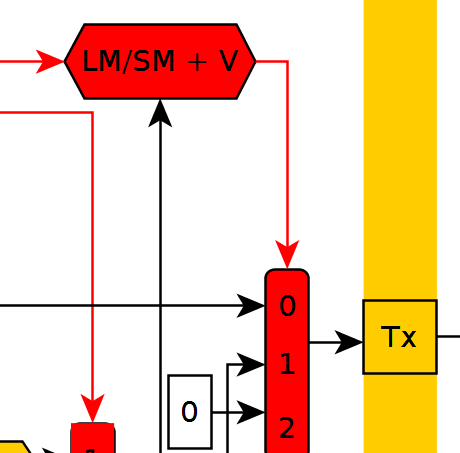
\includegraphics[scale=0.7]{lm_sm_init}


Initialisation logic:
    \begin{lstlisting}
        if(LM/SM == 0 && V == 0){
            Tx = 0;
        } else if(LM/SM == 1 && V == 0){
            Tx = Immediate;
        } else if(V == 1){
            Tx = Txn;
        }
    \end{lstlisting}

When V = 1, then \textbf{Wdis} is on for previous two pipeline registers and PC
so write is disabled and hence the next two instructions loaded are frozen in
fetch and decode stage.

\subsection*{PC update block}

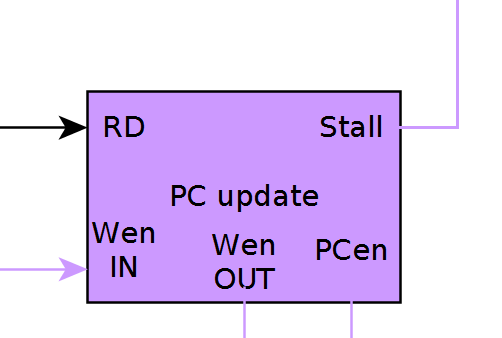
\includegraphics[scale=0.5]{pc}

\textbf{Stall} will make all stages \textbf{NOP} so that no instructions are executed,
and PC sets to branched value.
\textbf{WenOUT} will enable the PC branch mux to take from \textbf{Dwb}.
In normal case, \textbf{R7upd} enables writing of \textbf{PC} to \textbf{R7}.

Logic:
    \begin{lstlisting}
        if(NOP == 1){
            if(WenIN == 1 && RD == R7){
                R7upd = 0;
                WenOUT = 1;
                Stall = 1;
            } else {
                R7upd = 1;
            }
        }
    \end{lstlisting}


\subsection*{History Block}

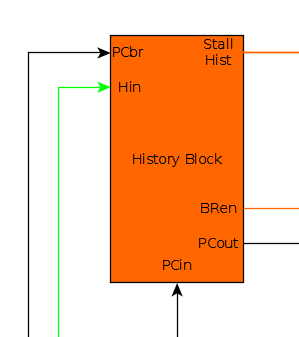
\includegraphics[scale=0.5]{history_block}

\textbf{PCin} is PC of the current fetched instruction.\\
\textbf{BRen} is output control signal to choose whether to update PC from
history table or not.\\
\textbf{PCout} is the next PC for current PC in history table.\\

\textbf{PCbr} is the PC of the \textbf{BEQ} instruction which may/may not branch.\\
\textbf{Hin} is the action that has been taken by that \textbf{BEQ} instruction.\\

\textbf{StallHist} is the control signal to flush and stall the pipeline if
history bit mismatched.

Internally, the \textbf{History Block} stores a history table with 
\textbf{PC\_curr},\textbf{PC\_next} and \textbf{H\_curr}.

We have used the same block for the implementation of \textbf{JAL} instruction since\\
this also deals with the static branch. The only difference is that we give the branch\\
decision as 1 always, since whenever \textbf{JAL} instruction appears we need to branch only.\\
This therefore saves one stall cycle for \textbf{JAL}.

Logic for \textbf{BRen},\textbf{PCout} and \textbf{StallHistory}:
    \begin{lstlisting}
        for(PC_curr,PC_next,H_curr in HistoryTable){
            if(PCbr == PC_curr){
                if(Hin != H_curr){
                    H_curr = Hin;
                    StallHistory = 1;

                    // PC+1 if Hin = 0, else BEQ will update directly
                    BRen = not(Hin);
                    PCout = PCbr + 1; 

                    break;
                }

            } else if(PCin == PC_curr){
                if(H_curr == 1){
                    BRen = 1;
                    PCout = PC_next;
                } else {
                    BRen = 0;
                }
            }
        }
    \end{lstlisting}


\section*{Control signals for each instruction}
\subsection*{ADD/NDU}

\begin{tabular}{|l|l|}
\hline
\textbf{Stage} & \textbf{Signals}\\
\hline
\textbf{Decode} & --\\
\hline
\textbf{Reg Read} & A1c = ra \\
                  & A2c = rb \\
                  & RDc = rc \\ 
\hline
\textbf{Exec} & ALU\_c = add/nand\\
              & Z = 1\\
              & C = 1(for add)\\  
\hline
\textbf{Mem} & --\\
\hline
\textbf{Write Back} & Wen = 1\\
                    & Cen = 1(for add)\\
                    & Zen = 1\\
\hline
\end{tabular}

\subsection*{ADC/ADZ/NDC/NDZ}
\begin{tabular}{|l|l|}
\hline
\textbf{Stage} & \textbf{Signals}\\
\hline
\textbf{Decode} & --\\
\hline
\textbf{Reg Read} & A1c = ra \\
                  & A2c = rb \\
                  & RDc = rc \\ 
\hline
\textbf{Exec} & ALU\_c = add/nand\\
              & Z = 1\\
              & C = 1(for add)\\
              & Flag = C/Z\\
\hline
\textbf{Mem} & --\\
\hline
\textbf{Write Back} & Wen = 1\\
                    & Cen = 1(for add)\\
                    & Zen = 1\\
\hline
\end{tabular}

\subsection*{ADI}
\begin{tabular}{|l|l|}
\hline
\textbf{Stage} & \textbf{Signals}\\
\hline
\textbf{Decode} & --\\
\hline
\textbf{Reg Read} & A1c = ra\\
                  & RDc = rb\\
\hline
\textbf{Exec} & ALU\_c = add\\
              & Z = 1\\
              & C = 1\\
              & Imm = 1\\
\hline
\textbf{Mem} & --\\
\hline
\textbf{Write Back} & Wen = 1\\
                    & Cen = 1(for add)\\
                    & Zen = 1\\
\hline
\end{tabular}

\subsection*{LHI}
\begin{tabular}{|l|l|}
\hline
\textbf{Stage} & \textbf{Signals}\\
\hline
\textbf{Decode} & LHI = 1\\
\hline
\textbf{Reg Read} & RDc = ra\\
\hline
\textbf{Exec} & LHI = 1\\
\hline
\textbf{Mem} & --\\
\hline
\textbf{Write Back} & Wen = 1\\
\hline
\end{tabular}

\subsection*{LW}
\begin{tabular}{|l|l|}
\hline
\textbf{Stage} & \textbf{Signals}\\
\hline
\textbf{Decode} & --\\
\hline
\textbf{Reg Read} & A1c = rb\\
                  & RDc = ra\\
\hline
\textbf{Exec} & ALU\_c = add\\
              & Imm = 1\\
\hline
\textbf{Mem} & LW = 1\\
             & MR = 1\\
             & Out\_c = 1\\
             & Zc = 1\\
\hline
\textbf{Write Back} & Wen = 1\\
                    & Zen = 1\\
\hline
\end{tabular}

\subsection*{SW}
\begin{tabular}{|l|l|}
\hline
\textbf{Stage} & \textbf{Signals}\\
\hline
\textbf{Decode} & --\\
\hline
\textbf{Reg Read} & A1c = rb\\
                  & A2c = ra\\
                  & Dmem = D2\\
                  & RM = A2\\
\hline
\textbf{Exec} & ALU\_c = add\\
              & Imm = 1\\
\hline
\textbf{Mem} & MW = 1\\
\hline
\textbf{Write Back} & -- \\
\hline
\end{tabular}

\subsection*{BEQ}
\begin{tabular}{|l|l|}
\hline
\textbf{Stage} & \textbf{Signals}\\
\hline
\textbf{Decode} & --\\
\hline
\textbf{Reg Read} & A1c = ra\\
                  & A2c = rb\\
\hline
\textbf{Exec} & BEQ = 1\\
              & ALU\_c = xor\\
\hline
\textbf{Mem} & --\\
\hline
\textbf{Write Back} & --\\
\hline
\end{tabular}


\subsection*{JAL}
\begin{tabular}{|l|l|}
\hline
\textbf{Stage} & \textbf{Signals}\\
\hline
\textbf{Decode} & JAL = 1\\
\hline
\textbf{Reg Read} & RDc = ra\\
\hline
\textbf{Exec} & ALU\_c = add\\
              & PC1 = 1\\
\hline
\textbf{Mem} & --\\
\hline
\textbf{Write Back} & Wen = 1\\
\hline
\end{tabular}

\subsection*{JLR}
\begin{tabular}{|l|l|}
\hline
\textbf{Stage} & \textbf{Signals}\\
\hline
\textbf{Decode} & --\\
\hline
\textbf{Reg Read} & RDc = ra\\
                  & A1c = rb\\
                  & JLR = 1\\
\hline
\textbf{Exec} & ALU\_c = add\\
              & PC1 = 1\\
\hline
\textbf{Mem} & --\\
\hline
\textbf{Write Back} & Wen = 1\\
\hline
\end{tabular}

\subsection*{LM}
\begin{tabular}{|l|l|}
\hline
\textbf{Stage} & \textbf{Signals}\\
\hline
\textbf{Decode} & LM/SM = 1\\
\hline
\textbf{Reg Read} & LM/SM = 1\\
                  & RDc = pe\\
                  & A1c = ra\\
\hline
\textbf{Exec} & ALU\_c = add\\
\hline
\textbf{Mem} & MR = 1\\
             & Out\_c = 1\\
\hline
\textbf{Write Back} & Wen = 1\\
\hline
\end{tabular}

\subsection*{SM}
\begin{tabular}{|l|l|}
\hline
\textbf{Stage} & \textbf{Signals}\\
\hline
\textbf{Decode} & LM/SM = 1\\
\hline
\textbf{Reg Read} & LM/SM = 1\\
                  & A2c = pe\\
                  & A1c = ra\\
\hline
\textbf{Exec} & ALU\_c = add\\
\hline
\textbf{Mem} & MW = 1\\
\hline
\textbf{Write Back} & --\\
\hline
\end{tabular}
\end{document}

